\documentclass[9pt,technote,compsoc]{IEEEtran}

% *** CITATION PACKAGES ***
%
\ifCLASSOPTIONcompsoc
  \usepackage[nocompress]{cite}
\else
  \usepackage{cite}
\fi

% *** GRAPHICS RELATED PACKAGES ***
%
\ifCLASSINFOpdf
\else
\fi

% correct bad hyphenation here
%\hyphenation{op-tical net-works semi-conduc-tor}
\usepackage[portuguese]{babel}
\usepackage[utf8]{inputenc}
\usepackage[table,xcdraw]{xcolor}
\usepackage{graphicx}
\usepackage{float}
\usepackage{booktabs}
\usepackage{tabularx}

\makeatletter
\renewcommand{\maketitle}{
\begin{flushleft}
  \LARGE{\textbf{\@title}}
  \normalsize{{\@author}}
\end{flushleft}
}
\makeatother

\begin{document}

\title{Relatório do Projeto 1 - Futoshiki}

\author{
Universidade de São Paulo - ICMC\\
\IEEEauthorblockN{\textbf{Aluno:} Jadson José Monteiro Oliveira\\}
\small{\IEEEauthorblockA{
\textbf{Número USP:} 10530309\\
\textbf{Email:} jadson@usp.br}\\
\textbf{Disciplina:} SCC5900}}

\maketitle

\IEEEpeerreviewmaketitle


\section{Introdução}
O projeto consiste na implementação de uma ferramenta que utilize uma abordagem backtracking para solucionar o Futoshiki, que é um jogo de tabuleiro cujo objetivo é preencher todas as variáveis com números, tal que nenhum dígito se repita em uma linha ou coluna, respeitando algumas restrições impostas, que informam se uma determinada variável deverá ser menor ou maior que outra variável adjacente.

Para solucionar esse problema, 3 metodologias, utilizando a abordagem de backtrack, foram implementadas e testadas. Nas Seções \ref{bt}, \ref{fc} e \ref{mrv}, o funcionamento de cada metodologia é descrito, na Seção \ref{experiments}, uma série de experimentos realizados é detalhada com o intuito de responder alguns questionamentos, e por fim, a Seção \ref{conclusion} descreve conclusões obtidas por meio da realização deste trabalho.


\section{Backtracking simples (BT)}\label{bt}
A primeira abordagem consiste na implementação básica de um algoritmo de BT, que não utiliza nenhuma heurística para realizar podas na árvore de possibilidades. Para isso, o tabuleiro foi representado como uma matriz \textbf{N} x \textbf{N}, onde \textbf{N} é a quantidade de linhas e colunas do tabuleiro. Para armazenar as restrições, utilizou-se uma estrutura de Hash, em que a complexidade de busca e armazenamento tende a ser constante ($O(1)$ e caso exista alguma colisão de hash, a linguagem de programação a trata de forma eficiente, onde o pior caso se torna $O(\log n)$).

O processo de resolução do problema utilizando esta abordagem é recursivo, percorrendo as colunas da matriz e realizando atribuições à primeira variável vazia, sendo que, os valores do domínio são recuperados sempre em ordem decrescente. Quando uma linha é completamente preenchida a busca é realizada na próxima linha, além disso, vale ressaltar que os valores válidos para atribuição respeitam todas as restrições impostas, portanto, não é possível preencher todo o tabuleiro com alguma restrição quebrada. O estado do tabuleiro é retornado a um anterior sempre que a árvore de possibilidades tenha atingido um nó folha sem solução. O procedimento é finalizado quando uma solução válida é encontrada, quando a quantidade de atribuições excede um limite de $10^{6}$ ou quando não existe uma solução válida para o tabuleiro definido, isto é, todas as possibilidades foram testadas dentro do espaço de $10^{6}$ atribuições.


\section{BT + Forward Checking (FC)} \label{fc}
FC é uma técnica de poda na árvore de possibilidades que verifica a existência de variáveis sem nenhum valor de domínio válido a cada atribuição (para uma variável qualquer), caso positivo, realiza o processo de backtrack (retorno), testando um outro valor de domínio para a variável pai (variável anterior). Esse procedimento é realizado até que uma solução seja encontrada, ou todas as possibilidades são testadas (com as podas realizadas), dentro de um limite estabelecido.

Para a implementação deste método de poda, utilizou-se uma estrutura auxiliar para atualização e recuperação dos valores válidos de domínio para cada linha e cada coluna. Essa estrutura auxiliar trata-se de um conjunto de bits para representar cada linha e cada coluna. Portanto, para a representação do estado do tabuleiro, utilizou uma matriz \textbf{(N+2)} x \textbf{N}, onde a linha \textbf{N+1} da matriz, é composta por \textbf{N} conjuntos de bits, cada um representando os valores utilizados em cada linha e a linha \textbf{N+2} da matriz, também composta por \textbf{N} conjuntos de bits, representando os valores utilizados em cada coluna.

\begin{figure}[H]
\centering{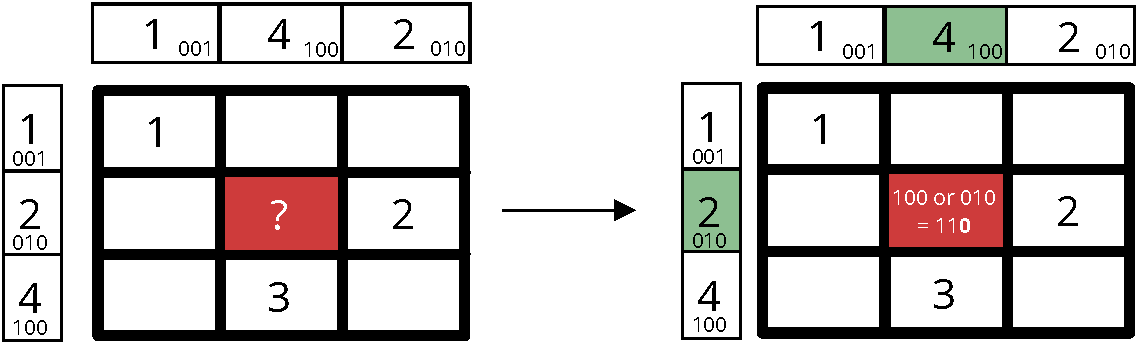
\includegraphics[width=8cm]{images/bitmask.pdf}}
\caption{Funcionamento da estrutura auxiliar com bits para recuperação de valores válidos na linha e coluna.}
\label{bitmask}
\end{figure} 

A Figura \ref{bitmask}, ilustra o processo de verificação dos valores válidos para determinada variável, onde o quadrado vermelho é a variável na qual se deseja saber quais os valores que ainda não foram utilizados em nenhuma linha ou coluna, para isso, é realizado uma operação de $or$ entre os bits da linha e da coluna da determinada variável, o resultado final é a exclusão dos valores que já estão utilizados. Esse procedimento otimiza o processo de verificação do domínio válido, realizando comparações em tempo constante. 


\section{BT + FC + Mínimos Valores Remanescentes (MRV)}\label{mrv}

MRV é uma outra técnica de poda, que visa diminuir o \textit{branching factor} da árvore de possibilidades. A técnica é aplicada na etapa de escolha da variável a ser preenchida, escolhendo a variável que tem a menor quantidade de valores válidos no domínio. Neste projeto, 3 variações do MRV foram implementadas e testadas, a heurística também utiliza a estrutura auxiliar descrita na Seção \ref{fc} e os resultados experimentais estão descritos na Seção \ref{experiments}.

A primeira implementação do MRV (MRV$_{1}$), baseiou-se na definição padrão da heurística, onde a variável escolhida deve ser aquela que tem a menor quantidade de valores válidos no domínio, verificando tanto a condição de dígito exclusivo na linha e coluna como respeitando as restrições de menor e maior. Para o caso de ocorrer empate na quantidade de valores válidos, a primeira variável (na sequência linha e coluna) é escolhida.

A segunda implementação do MRV (MRV$_{2}$), utilizou somente a condição de exclusividade para a linha e coluna, para contagem de valores válidos. Para o caso de ocorrer empate na quantidade de valores válidos, a primeira variável (na sequência linha e coluna) é escolhida.

A terceira implementação do MRV (MRV$_{3}$), utilizou a primeira implementação com a adição da heurística Grau como critério de desempate, quanto maior o grau da variável (maior quantidade de restrições), maior a sua prioridade na escolha.

\section{Resultados Experimentais}\label{experiments}

Uma série de experimentos foram realizados com o intuito de responder as seguintes questões:

\begin{itemize}
\item A implementação do BT + MRV$_{1}$ + FC está correta?
\item Levando em consideração o tempo de execução e a quantidade de atribuições para cada algoritmo, qual o custo/benefício de utilizar heurísticas para realizar podas na árvore de possibilidades?
\item A quantidade de atribuições necessárias para solucionar o problema é influenciada pela quantidade de restrições do problema?
\end{itemize}

As próximas seções esclarecerão todos esses pontos, os experimentos foram realizados utilizando a linguagem de programação Java, e testadas em um computador \textit{Intel Core 2 Quad CPU Q9550 @ 2.83GHz com 4 núcleos} e foram avaliadas a partir de um conjunto de casos de testes (futoshiki\_all, mrv\_only, arc\_consistent, arc\_inconsistent), disponibilizados pelos docentes da disciplina.

\subsection{Corretude do BT + MRV$_{1}$ + FC}

O principal objetivo deste experimento é a validação do método de poda MRV$_{1}$, para isso, utilizou-se o conjunto de entradas \textit{mrv\_only}. O arquivo é composto por 60 casos de teste e todos eles são solucionáveis utilizando o método BT + MRV$_{1}$ + FC, além de que a quantidade de atribuições de variáveis para encontrar uma solução deve ser exatamente igual à quantidade de variáveis inicialmente não preenchidas. O resultado para este experimento foi o esperado, provando que a implementação do método MRV$_{1}$ está correta.

\subsection{Custo/benefício para utilização dos métodos de poda}

Para analisar o custo/benefício para utilização dos métodos de poda, utilizou-se os conjuntos de casos de teste \textit{mrv\_only}, \textit{arc\_consistent} e \textit{arc\_inconsistent}. Cada heurística foi executada 5 vezes em cada conjunto de testes e a média de tempo total foi extraída, bem como a quantidade de casos resolvidos e a soma das atribuições realizadas para todo o conjunto, conforme demonstrado na Tabela \ref{table1}.

\newcolumntype{L}[1]{>{\raggedright\arraybackslash}p{#1}}
\newcolumntype{C}[1]{>{\centering\arraybackslash}p{#1}}
\newcolumntype{R}[1]{>{\raggedleft\arraybackslash}p{#1}}

\begin{table}[H]
\centering
\caption{Comparativo entre os métodos implementados}
\label{table1}
\begin{tabular}{|l|c|c|c|}
\hline
\textbf{Método utilizado} & \multicolumn{1}{l|}{\textbf{Segundos}} & \multicolumn{1}{l|}{\textbf{Soluções}} & \multicolumn{1}{l|}{\textbf{Atribuições}} \\ \hline
\multicolumn{4}{|c|}{\textbf{Arquivo de casos de teste: mrv\_only}} \\ \hline
BT & 0.006 & \textbf{60} & 1.660 \\ \hline
\rowcolor[HTML]{9AFF99} 
BT + FC & \textbf{0.005} & \textbf{60} & 1.497 \\ \hline
\rowcolor[HTML]{9AFF99} 
BT + MRV$_{1}$ + FC & 0.008 & \textbf{60} & \textbf{1.312} \\ \hline
BT + MRV$_{2}$ + FC & 0.006 & \textbf{60} & 1.320 \\ \hline
\rowcolor[HTML]{9AFF99} 
BT + MRV$_{3}$ + FC & 0.020 & \textbf{60} & \textbf{1.312} \\ \hline
\multicolumn{4}{|c|}{\textbf{Arquivo de casos de teste: arc\_consistent}} \\ \hline
BT & 1.439 & 57 & 7.792.205 \\ \hline
BT + FC & 1.568 & 58 & 5.026.495 \\ \hline
\rowcolor[HTML]{9AFF99} 
BT + MRV$_{1}$ + FC & \textbf{0.105} & \textbf{60} & \textbf{13.786} \\ \hline
BT + MRV$_{2}$ + FC & 0.588 & \textbf{60} & 262.233 \\ \hline
BT + MRV$_{3}$ + FC & 0.170 & \textbf{60} & 15.012 \\ \hline
\multicolumn{4}{|c|}{\textbf{Arquivo de casos de teste: arc\_inconsistent}} \\ \hline
BT & \textbf{1.884} & 51 & 10.228.149 \\ \hline
BT + FC & 2.700 & 52 & 9.574.504 \\ \hline
\rowcolor[HTML]{9AFF99} 
BT + MRV$_{1}$ + FC & 5.182 & \textbf{59} & \textbf{1.420.255} \\ \hline
BT + MRV$_{2}$ + FC & 19.270 & 52 & 8.708.727 \\ \hline
BT + MRV$_{3}$ + FC & 16.749 & 58 & 2.539.032 \\ \hline
\end{tabular}
\end{table}

A Tabela \ref{table1} apresenta os resultados obtidos pelos métodos implementados. A primeira coluna da tabela, informa qual o método utilizado, a segunda coluna da tabela informa o tempo gasto em segundos para executar todo o conjunto de casos de teste, a terceira coluna exibe a quantidade de soluções encontradas e a última coluna representa a quantidade total de atribuições.

É possível observar que, de modo geral, o método BT + MRV$_{1}$ + FC obteve os melhores resultados, mesmo necessitando realizar operações adicionais sobre o BT normal, a drástica redução na quantidade de atribuições beneficiou o tempo de execução do algoritmo, viabilizando a utilização deste para solucionar casos mais pesados, com soluções mais difíceis de serem encontradas, consequentemente o custo/benefício de se utilizar esta poda, neste problema específico, é consideravelmente alto.
\subsection{Influência da quantidade de restrições na busca de uma solução para o tabuleiro}

Um dos principais pontos críticos para resolver o problema do Futoshiki é a busca por estados do tabuleiro que não quebre as restrições impostas. Este experimento teve como objetivo analisar se existe uma influência entre a quantidade de restrições e a dificuldade de encontrar uma solução para o problema. Para isto, o conjunto de casos de teste \textit{futoshiki\_all} foi utilizado, a partir de então, todos os casos de teste com tabuleiros 6x6 foram selecionados, sendo que esses casos específicos tem diferentes quantidades de restrições. A metodologia BT + MRV + FC, foi utilizada para solucionar os casos de testes especificados, obtendo resultados que estão ilustrados na Figura \ref{constraints}.

\begin{figure}[H]
\centering{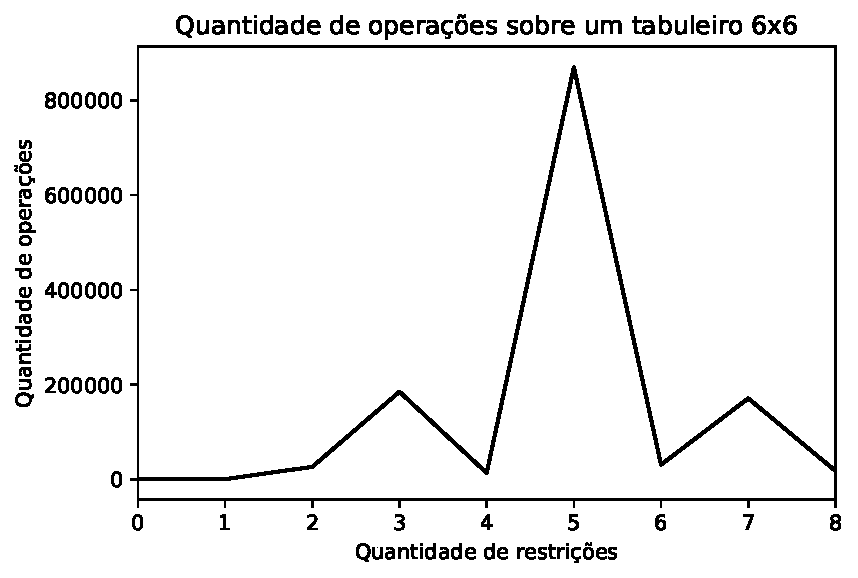
\includegraphics[width=8cm]{images/constraints.pdf}}
\caption{Influência da quantidade de restrições para a busca de uma solução.}
\label{constraints}
\end{figure}

Observando a Figura \ref{constraints}, percebe-se que existe um comportamento peculiar em relação à quantidade de restrições e a quantidade de operações necessárias para encontrar uma solução em tabuleiros com a mesma quantidade de linhas e colunas (neste caso, 6x6). Baseado neste resultado, podemos afirmar que é necessário um nivelamento entre a quantidade de restrições e a quantidade de variáveis do tabuleiro, para que o problema se torne consideravelmente complicado de se resolver, isto é, uma quantidade de restrições muito pequena ou muito grande, pode tornar um tabuleiro do Futoshiki mais fácil de se resolver computacionalmente.

\section{Conclusão}\label{conclusion}

Conclui-se que apesar do esforço adicional gerado pelas verificações na tentativa de realizar podas, experimentos realizados neste projeto, demonstram que este esforço é compensado pela redução da quantidade de atribuições nas variáveis do tabuleiro. Outro fato interessante é que a quantidade de restrições no tabuleiro influencia na quantidade de atribuições necessárias, ou seja, um caso de teste que tenha poucas ou muitas restrições, pode tornar o problema mais fácil de se resolver computacionalmente. Por fim, existem inúmeras metodologias para realizar podas na árvore de possibilidades, mas é necessário realizar análises em relação ao custo/benefício de utilização desses métodos, pois geralmente eles requerem esforços e verificações adicionais, o que pode inviabilizar a busca por uma solução do problema.

\end{document}

